%!TEX root = mb.tex



\section{Cryptographic Building Blocks}
\label{sec:buildingblocks}

In this section we present the building blocks \sys relies on.
AES is a well known encryption technique and we do not discuss it here. Instead, we briefly discuss keyword match (introduced by~\cite{blindbox}, to which we refer the reader for details) and more extensively discuss range match, a new cryptographic scheme we designed for this setting.
When describing these schemes we refer to the encryptor as the gateway whose secret key is $k$ and to the entity computing on the encrypted data as the service provider (SP).


\subsection{KeywordMatch}\label{s:kwmatch}


KeywordMatch allows detecting if an encrypted keyword matches an encrypted data item by equality.
For example, given an encryption of the keyword ``malicious'', and a list of encrypted strings  [$\Enc$(``alice''), $\Enc$(``malicious''), $\Enc$(``alice'')], SP can  detect that the keyword matches the second string. 
For  this, we use a searchable encryption scheme~\cite{song:search, blindbox}.
Using this scheme, the gateway can encrypt a value $v$ into $\enc(v)$ and a rule $r$ into $\encr$ and SP can detect if there is a match between $v$ an $r$. 
 The security of searchable encryption is well studied~\cite{song:search, blindbox}: at a high level,  given a list of encrypted strings, and an encrypted keyword, SP does not learn anything about the encrypted strings, other than which strings match the keyword. 
 The encryption of the strings is {\em randomized}, so it does not leak whether two encrypted strings are equal to each other, unless, of course, they both match the encrypted keyword. 
  We use the technique from~\cite{blindbox}.

%!TEX root = mb.tex

%\section{Building block: Range match}
%An important operation over an encrypted packet is to determine if an encrypted field in the packet falls in an encrypted range.
%We will use the firewall as an example. 
%Consider the following firewall rule:
%
%Constructing an encryption scheme that allows checking if an encrypted value is in an encrypted range, has been a challenge in the applied cryptography community. The reason is that ..
%
%\begin{itemize}
%\item preserve the order between Encryptd values
%\item candidate: OPE
%\item candidate: mOPE
%\item So none of the existing schemes are satisfactory. A new scheme \RM.
%\end{itemize}
%
%\RM applies to cases when we know an upper bound on the values encrypted with OPE and this is a small number of values (say, less than 10,000).
%
%The small number of values permits us to improve in two ways over mOPE [1]
%No more interaction. We store the tree in mOPE on the gateway (client) side, which means that the gateway can compute a new encryption by itself without help from service provider. The storage at the gateway will remain small.
%Rare updates to ciphertexts. We can space out the ciphertexts of the values encrypted sufficiently. 
%
%This also enjoys a stronger security than OPE! It leaks less than order.
%The reason is that, the server does not learn the order between the values in packets, and only whether they map between two values in the rules. 
%
%this one is new
%
%discuss 
%
%would be good to explain the challenge from the 
%
%\todo{a more interesting name to the scheme}
%
%prefix gets mapped into interval, at most a certain number
%
%talk about building certain data structures that all works the same
%
%firewall need not change 

\subsection{Range match } \label{sec:range}

Many middleboxes perform detection over a {\it range} of port numbers or IP addresses. For example, a network administrator might wish to block access to all servers hosted by Stanford, in which case the administrator would block access to the network prefix 18.0.0.0/8, \ie{}, 18.0.0.0-18.255.255.255. RangeMatch enables a middlebox to tell whether or not an IP address $v$ lines in between such a range $[s_1, e_1]$, where $s_1$ = 18.0.0.0 and $e_1$ = 18.255.255.255; however, the middlebox does not learn the values of $v$, $s_1$, or $e_1$.
Unlike KeywordMatch (or AES), RangeMatch is a new scheme we designed specifically for our setting.

One might ask whether RangeMatch is strictly necessary. To detect whether or not a port number lies in the range 80-83 is the same as asking whether the port number is equal to anything in the set \{80,81,82,83\} -- hence, one could use KeywordMatch to implement all range detection operations by converting each range to a set of exact-match values.
However, in practice, the overhead of doing this is prohibitive.
For our own department network, doing so would convert our IPv6 and IPv4 firewall rule set of only 97 range-based rules to $2^{238}$ exact-match only rules; looking only at IPv4 rules would still lead to 38M exact-match rules.
Hence, to perform typical middlebox behaviors {\it in practice}, we require a RangeMatch scheme which is more efficient.

\subsubsection{Requirements}
The functionality of our RangeMatch scheme is to encrypt a set of ranges $[s_1, e_1]$, $\dots$, $[s_n, e_n]$ into  $[\Enc(s_1)$, $\Enc(e_1)]$, $\dots$, $[\Enc(s_n)$,  $\Enc(e_n)]$, and a value $v$ into $\Enc(v)$, such that anyone with access to these encryptions can determine in which range $v$ lies, while not learning the values of $s_1$, $e_1$, $\dots$, $s_n$, $e_n$, and $v$. 
For concreteness, we explain our scheme by considering $v$, $e_i$ and $s_i$ as IP addresses (although it can be used for encrypting ports too).

Our goal in designing RangeMatch was for it to be both efficient/fast {\em and} provides strong security.

In terms of performance, both encryption (performed at the gateway) and detection (performed at the middlebox) should be practical for typical middlebox line rates.
Our RangeMatch encrypts in $< 3\mu$s per value (we evaluate in \S\ref{sec:eval}).
Our design performs comparison between encrypted values and an encrypted rule (performed at the middlebox) using only on normal $\leq$/$\geq$ operators; hence it is compatible with existing classification algorithms such as tries, area-based quadtrees, FIS-trees, or hardware-based algorithms~\cite{packet_classif}.

For security, we require that the encryption scheme  not leak $v$, $e_1$, $s_1$, $\dots$, $e_n$, $s_n$ to SP.
Ideally, SP does not learn anything about $v$ other than what interval it matches to. In  particular, even if $v_1$ and $v_2$ match the same range, SP should not learn their order. SP is allowed to learn the order relation of the intervals (in fact, in many setups, SP provides the intervals). 
RangeMatch is the only scheme we know of to provide this security guarantee.

Although RangeMatch is similar to order-preserving encryption such as BCLO~\cite{boldyreva:ope} or mOPE~\cite{popa:mope}, neither meets our security requirement (because they leak the ordering between encrypted values, not just their ordering relative to rules), and neither provides the performance necessary for packet processing (as we show in \S\ref{sec:eval}).

\eat{
\begin{CompactEnumerate}[leftmargin=*]

\item  {\em be fast}: the throughput of encryption should be not much lower than network throughput. In particular, the scheme should preserve the ability to use {\em existing fast packet matching algorithms}, such as  various kinds of tries, area-based quadtrees, FIS-trees, or hardware-based algorithms~\cite{packet_classif}.  All of these rely on the ability of SP  to compute ``>'' between $v$ and the endpoints of an interval,
hence the encryption scheme should preserve this property. 

\item {\em provide strong security}: The encryption scheme should not leak $v$, $e_1$, $s_1$, $\dots$, $e_n$, $s_n$ to SP.
Ideally, SP does not learn anything about $v$ other than what interval it matches to. In  particular, even if $v_1$ and $v_2$ match the same range, SP should not learn their order. SP is allowed to learn the order relation of the intervals (in fact, in many setups, SP provides the intervals). \label{req:sec}

\item {\em be deterministic}: To integrate with NAT and to enable middleboxes to piece together packets from the same flow, each value should get  consistently  the same encryption. Any changes in the encryption assigned should happen rarely.  \label{req:injective}

\item {\em be format-preserving}: The encryption should have the same format as the data. Concretely, an encrypted IP address should look like an IP address.  This property is important to avoid changing the packet header structure, which would be a hurdle to adoption. 
 \end{CompactEnumerate}
}


\subsubsection{Our RangeMatch scheme} 



%We explain the scheme based on encryption IP addresses for a firewall and source IP addresses in packets, although the scheme is used in encryption other fields too, as explained in Sec.~\ref{xx}.

To encrypt the endpoints of the intervals, we sort them, and choose as their encryptions values equally distributed in the domain space in a way that preserves the order of the endpoints. For example, the encryption of the intervals 127.0.0.0/8 and 172.16.0.0/16, is [51.0.0.0, 102.0.0.0] and [153.0.0.0, 204.0.0.0]. This preserves the order of the intervals but does not leak anything else.

For now, consider that the gateway  maintains a mapping of each interval endpoint  to its encryption, called the {\em interval map}.  The interval map also contains the points $- \infty$ and $+ \infty$, encrypted with 0.0.0.0 and 255.255.255.255. 


When the gateway needs to encrypt an IP address $v$, the gateway first determines what  is the interval  $v$ falls in (we discuss below what happens when more than one interval matches). It uses the interval map to determine the encryptions of the endpoints of this interval. Then, to encrypt $v$, it chooses a random value in this interval.
For example, if $v$ is 127.0.0.1, a possible encryption is 48.124.24.85. The encryption does not retain any information about $v$ other than the range it is in. In particular, for two values $v_1$ and $v_2$ that match the same interval, SP does not learn their order. Thus, this satisfies the security requirement above.

\begin{figure}[t]
  \centering
  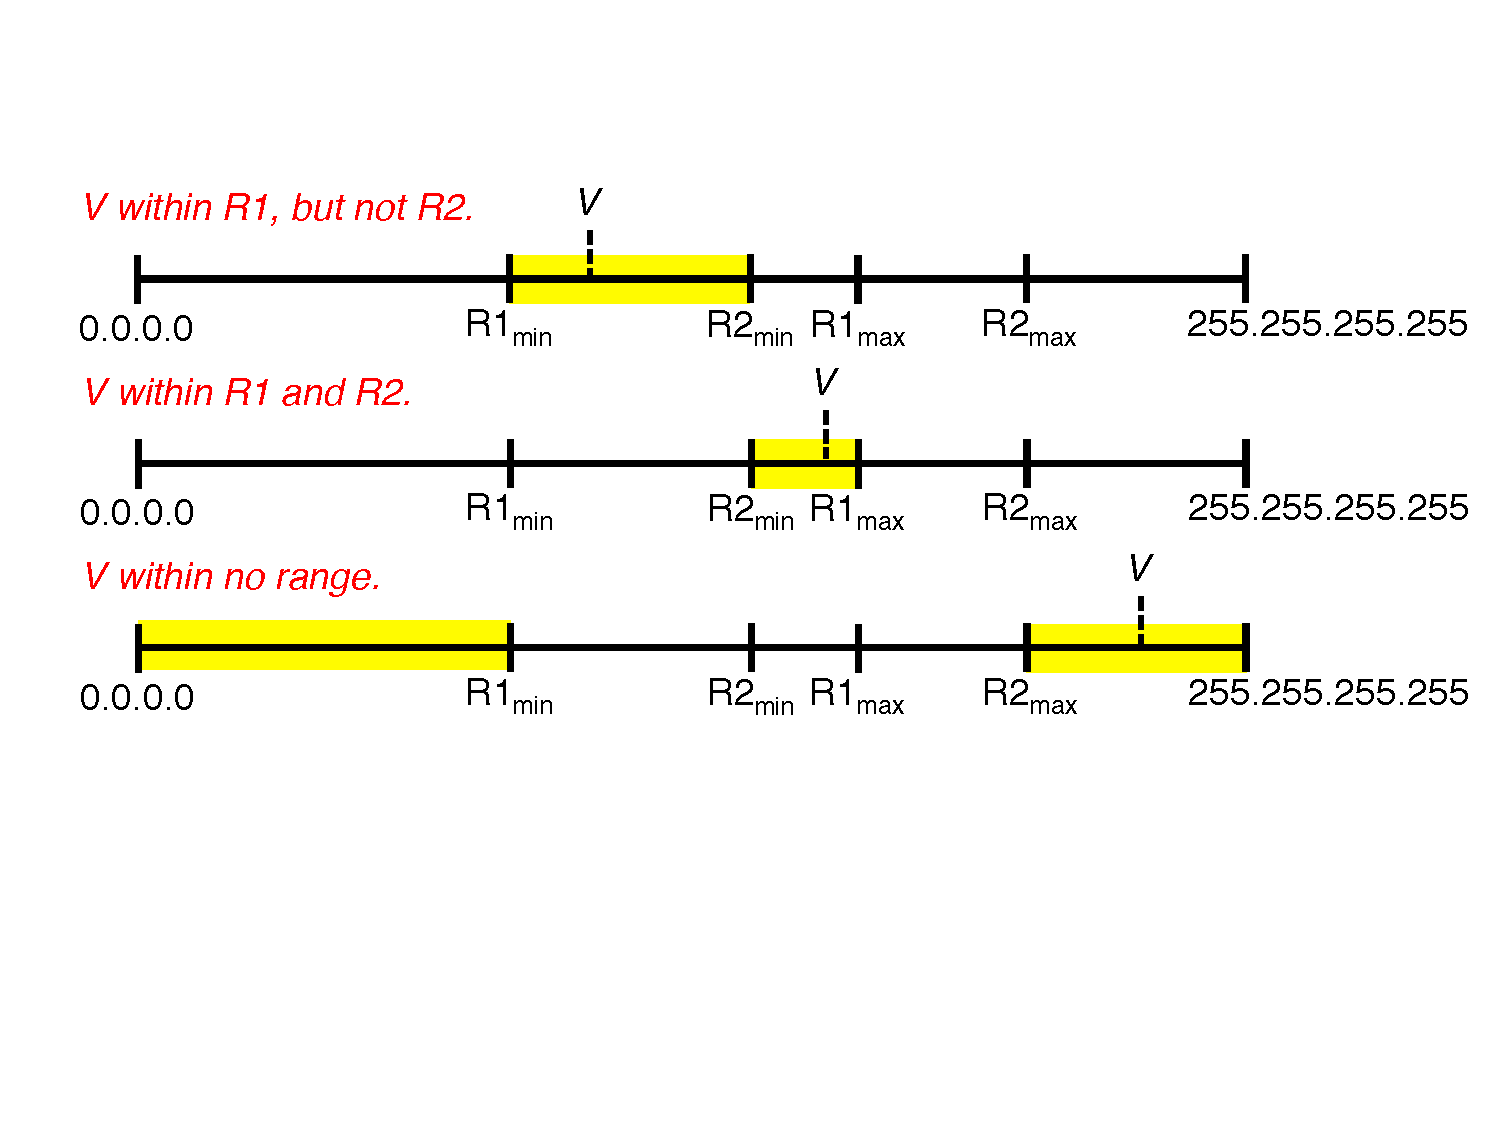
\includegraphics[width=3.25in]{fig/rangeopts.pdf}
  \caption[]{Possible RangeMatch encryption values.\label{fig:rangeopts}}
\end{figure}
To generalize this insight, we need to specify how to encrypt $v$ when $v$ fits in multiple intervals or in no interval at all. Figure~\ref{fig:rangeopts} illustrates how $v$ is mapped depending on whether it maps to zero, one, or both of ranges $R1$ and $R2$; we formalize this as follows. 

To achieve the desired security, the we find interval $I$ (which may consist of many sub-intervals, \eg{} when $v$ matches neither $R1$ or $R2$ in Fig.~\ref{fig:rangeopts}) inside which $v$ should be mapped at random. The equation for $I$ is as follows. Consider the intervals {\em inside} which $v$ falls, and let $I_0, I_1, \dots, I_{n_I}$ be their encryptions. We always include the total interval $I_0 = [0.0.0.0, 255.255.255.255]$. Now consider the intervals {\em outside} of which $v$ falls and let $O_1, \dots, O_{n_O}$ be their encryptions. Then, to provide our desired security goal, $v$ should be chosen at random from the interval  
\begin{equation}
 I = I_0 \cap I_1 \cap ... \cap I_{n_I} - (O_1 \cup \dots \cup O_2). \label{eq:randominterval}
 \end{equation}

 

To support middleboxes like NATs -- which require that every time a value for the same connection is encrypted, it return the same value -- we need to generate the random encryptions using a deterministic function. Importantly, this value should always be the same {\it within} the same connection, but across different connections it should be different. For this, we use a pseudorandom function~\cite{GoldreichVol1}, $\prf$. Let $\prf$ be a function $\prf^{x}(n) \rightarrow {1 \ldots x}$, mapping $n$ to a random value between $1$ and $x$ inclusive. 

We seed $\prf$  in $q$, a function of both the key and hash of the 5-tuple connection header ($q = \prf_k(\text{conn})$).  Let $|I|$ be the size of the interval $I$. 
Then, the encryption of $v$ is the $\mathsf{index}$-th element in $I$, where $\mathsf{index}$ is 
%\[ \mathsf{index}(v) = \prf_k(v)\ \mod\ |I|. \] 
\[ \mathsf{index}(v) = \prf_{q}^{|I|}(v) \] 
  Note that, in the systems setup with two gateways, the gateways generate the same encryption because they share $k$. 

When encrypting IP addresses, we do not want two different IP addresses to map to the same encryption (which would break the NAT). Fortunately, the probability that two IP addresses get assigned to the same encryption is negligibly low for IPv6. This probability is very low for IPv4, but not low enough that a collision will not happen in a large interval of time. The reason is that each interval of encryptions is large because we distributed the endpoint encryptions evenly and because there is a small number of such endpoints in a realistic setting (e.g., a firewall has less than 100,000 rules). Suppose we have $n$ distinct rules, $m$ flows and a $w$-bit space, the probability of getting collision is approximately $1-e^\frac{-m^2 (n+1)}{2^{w+1}}$. Therefore, if $w=128$ (which is the case when we use IPv6), the probability is negligible in a normal setting. 
\begin{figure}
  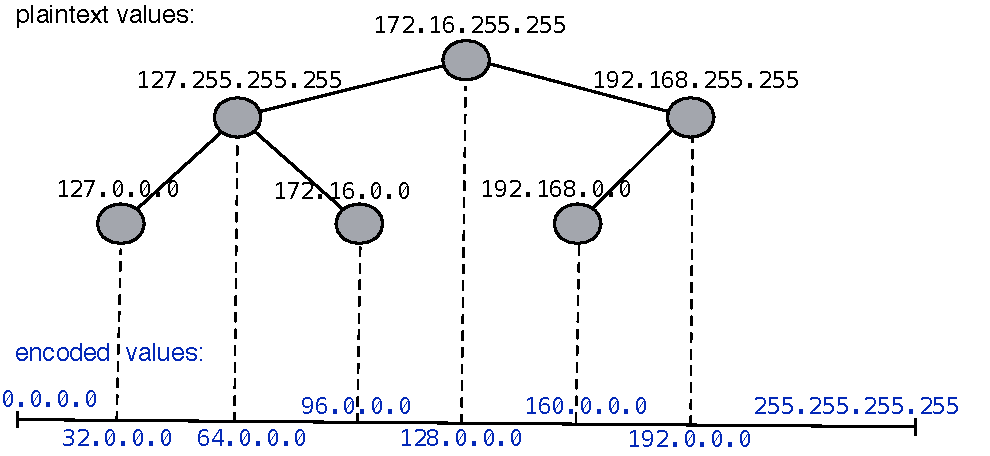
\includegraphics[width=3.45in]{fig/tree}
  \caption{\label{fig:tree} Range match tree. The values of nodes in the tree are the unencrypted IP addresses, and the blue values on the horizontal axis are their encryptions. }
\end{figure}

\textbf{Comparing encrypted values against rules.}
The cloud can run ``$\ge$'' and ``$\le$" between any encrypted value $\enc(v)$ and an encrypted endpoint $\enc(s)$ and $\enc(e)$, and will obtain a correct answer. Computing $\enc(v_1) < \enc(v_2)$  between two encrypted values in the same range is meaningless, and returns a random value.





\textbf{Security guarantees.}
The scheme achieves our desired security goal: the only information leaked about a value $v$ encrypted is which ranges it matches. 
In particular, the scheme is not order preserving because it does not leak the order of two encrypted values that match the same range. It is easy to check that the scheme is secure: since the encryption of $v$ is random in $I$ (Eq.~\ref{eq:randominterval}), the scheme only leaks the fact that $v$ is in $I$. $I$ is chosen in such a way that the only information about $v$ it encodes is which intervals $v$ matches and which it does not match.

\subsubsection{Implementing RangeMatch in the Gateway}
\label{sec:tree}
To encrypt using RangeMatch, the gateway must store a tree -- as shown in Figure~\ref{fig:tree} -- mapping the unencrypted intervals to the encrypted address space.
%Most encryption operations are relatively stateless -- they rely only on the key and the data. Using RangeMatch requires that the Rule Encryption component manage a tree of values for use at encryption time; we discuss how this tree is generated now.

The gateway keeps a small amount of state (in our implementation, about 200 bytes/range) encryption the intervals, but maintains no state per IP address encrypted or per connection. The gateway stores the tree in Fig.~\ref{fig:tree}: for each node, it stores the unencrypted endpoint, whether it is the left or  right margin of an interval, and the other endpoint of the interval it is part of. It does not need to store the encryption of the endpoint because this is easy to derive from the position in the tree. 


The gateway can use the following functions. EncryptRanges encrypts the initial ranges. Note that some ranges could consist of
one point only, namely $s = e$. 

% TO CUT TO REDUCE: put all these algorithms into one box
% framed takes space around it, above it, below it 

\begin{framed}
\begin{algorithmic}[1]

\Procedure{EncryptRanges}{[$s_1$, $e_1$], $\dots$, [$s_n$, $e_n$]}
  \State Build scapegoat tree on the values 
              $\{s_1, \dots, s_n\}$ 
              $\cup$ $\{e_1, \dots, e_n\}$ 
              $\cup$ $\{-\infty, \infty\}$.
  \State Assign an encryption $\enc(x)$ to each node $x$ in the tree:
  \begin{itemize}
  \item the root gets the middle of the IP range, $e$, 
  \item the node to the left of the root gets the middle of the interval to the left of $e$: ($e/2$),
  \item the right node gets the middle of the range
  to the right of $e$: ($3e/2$), and so on.
  \end{itemize}

  \State \Return{[$\enc(s_1)$, $\enc(e_1)$], $\dots$, [$\enc(s_n)$, $\enc(e_n)$]}
\EndProcedure

\end{algorithmic}
\end{framed}



EncryptValue encrypts the values to be matched against ranges.

\begin{framed}
\begin{algorithmic}[1]

\Procedure{EncryptValue}{$v$}
  \State Search the tree for $v$ to compute efficiently I as in Eq.~\ref{eq:randominterval}.
  \State Compute $\mathsf{index}(v) = \prf_k(v)\ \mod\ |I|.$ 
  \State Let $\enc(v)$ to be the $\mathsf{index}$-th element of $I$. 
  \State \Return $\left(\enc(v), \IV, \aes_k(\IV, v)\right)$ for random $\IV$. 
\EndProcedure

\end{algorithmic}
\end{framed}

Here is how to compute $I$ efficiently. When searching for $v$ in the tree, the gateway
can identify the tightest enclosing interval [$p_1$, $p_2$] in logarithmic time. 
 If $[p_1, p_2]$ are endpoints of the
same interval, then I = [$p_1$, $p_2$]. Otherwise, move towards the left in the tree until you identify the first endpoint
$\ell_1$
that belongs to an interval $[\ell_1, \ell_2]$ enclosing $v$. Then, using the tree, scan $[\ell_1, \ell_2]$ and eliminate
any intervals not containing $v$. The gateway can precompute and store this interval for every two consecutive nodes in the tree.

EncryptValue returns an AES encryption of $v$ too, because $\enc(v)$ is not decryptable. 

We now describe the procedure for AddRange and DeleteRange which add or delete an interval. 
These will modify the state at the gateway. Besides the interval added or deleted, a small number
of other intervals may be moved -- at worst, $O(\log n)$. For these, the algorithm returns the old and new encryption of the interval. 


\begin{framed}
\begin{algorithmic}[1]

\Procedure{AddRange}{$[s, e]$}
  \State Insert $s$ and $e$ into the scapegoat tree. If $s=e$, insert the value only once.
  %	
  \State Initialize $L$ to be the empty list.
  \If{tree needs to be rebalanced}
  	\State Record which nodes change position in the tree during rebalancing, together with 
	their old and new encryptions. Namely, record	\[L = \{ \en_1 \leftarrow \en^*_1, \dots, \en_m \rightarrow \en^*_m\},\] where $m$ is the number of nodes who changed position in the tree, and $\en_i$ and $\en^*_i$ are the old and new encryption of the $i$-th node that changed position. 
  \EndIf
  \State Compute  $\enc(s)$ and $\enc(e)$, the encryptions of $s$ and $e$, as in EncryptRanges.
   \State \Return{$[\enc(s), \enc(e)], L$}
\EndProcedure

\end{algorithmic}
\end{framed}

%  \State Determing the smallest and the largest encryption in the values $[\enc(s), \enc(e)]$ and $L$, and call this $\dirtyrange$.

Since we are using a scapegoat tree, the number of nodes that change position during rebalancing is amortized worst case $O(\log n)$ where $n$ is the total number of nodes in the scapegoat tree. 

DeleteRange is similar, except that the result contains only $L$. 

\subsubsection{Rule Updates at the Cloud}
\label{sec:updates}
At the cloud, RangeMatch poses two additional challenges to updating rules, both stemming from the fact that a rule update also will change encrypted values within packets.
The first challenge is middlebox state. Consider a NAT with a translation table containing ports and IP addresses for active connections. 
Adding or removing a rule will modify some $\log(n)$ of these values in the RangeMatch tree, and thus to continue correct processing the NAT state must correspondingly be updated.
The second challenge is a race condition: when the middlebox adopts a new ruleset while packets encrypted under the old tree are still flowing, these packets will be misclassified as their encryption values are inconsistent with the ruleset being applied. 
The same problem occurs if packets encrypted under the new tree arrive before the new rulset has been adopted.

When the RangeMatch tree is updated, the gateway and cloud provider do the following to avoid these problems. 
When the gateway updates the RangeMatch tree it announces to the cloud provider of the pending update, and the middleboxes ship their current state to the gateway to receive the new encryption values.
The gateway then sends a signal to the cloud provider that it is about to `swap in' the new tree. 
The cloud provider buffers traffic for a few hundred milliseconds after this signal to allow all old traffic to complete processing at the cloud; it signals to all middleboxes to `swap in' the new rules and state; and once all of this is completed it allows the new traffic to flow through the network and receive processing under the new policy.
Note that all changes to middleboxes are in the {\it control plane} of the middlebox, and require no modifications to the algorithms and operations performed in per-packet processing.
